%!TeX program = xelatex
\documentclass{SYSUReport}
\usepackage{tabularx} % 在导言区添加此行
\usepackage{listings}
\usepackage{xcolor}
\usepackage{float}

\lstset{
    basicstyle=\ttfamily\small,    % 基本字体
    keywordstyle=\color{blue},     % 关键字颜色
    commentstyle=\color{green},    % 注释颜色
    stringstyle=\color{red},       % 字符串颜色
    numbers=left,                  % 显示行号
    numberstyle=\tiny\color{gray}, % 行号样式
    frame=single,                  % 边框样式(single, shadowbox等)
    breaklines=true,               % 自动换行
    tabsize=4                      % Tab缩进长度
}

% 根据个人情况修改
\headl{}
\headc{}
\headr{并行程序设计与算法实验}
\lessonTitle{并行程序设计与算法实验}
\reportTitle{Lab0-环境设置与串行矩阵乘法}
\stuname{林隽哲}
\stuid{21312450}
\inst{计算机学院}
\major{计算机科学与技术}
\date{\today}
\setlength{\headheight}{15pt}

\begin{document}

% =============================================
% Part 1: 封面
% =============================================
\cover
\thispagestyle{empty} % 首页不显示页码
\clearpage

% % =============================================
% % Part 4: 正文内容
% % =============================================
% % 重置页码,并使用阿拉伯数字
% \pagenumbering{arabic}
% \setcounter{page}{1}

%%可选择这里也放一个标题
%\begin{center}
%    \title{ \Huge \textbf{{标题}}}
%\end{center}

\section{实验目的}
\begin{itemize}
   \item 理解并行程序设计的基本概念与理论。
    \item 掌握使用并行编程模型实现常见算法的能力。
    \item 学习评估并行程序性能的指标及其优化方法。
\end{itemize}

\section{实验内容}
\begin{itemize}
    \item 设计并实现以下矩阵乘法版本:
    \begin{itemize}
        \item 使用C/C++语言实现一个串行矩阵乘法。
        \item 比较不同编译选项、实现方式、算法或库对性能的影响:
        \begin{itemize}
            \item 使用Python实现的矩阵乘法。
            \item 使用C/C++实现的基本矩阵乘法。
            \item 调整循环顺序优化矩阵乘法。
            \item 应用编译优化提高性能。
            \item 使用循环展开技术优化矩阵乘法。
            \item 使用Intel MKL库进行矩阵乘法运算。
        \end{itemize}
    \end{itemize}
    \item 生成随机矩阵A和B,进行矩阵乘法运算得到矩阵C。
    \item 衡量各版本的运行时间、加速比、浮点性能等。
    \item 分析不同实现版本对性能的影响。
\end{itemize}

\section{实验结果}

我当前使用的CPU为Intel 酷睿 i5 12490,拥有6核心12线程,CPU主频3GHz,最高睿频4.6GHz。浮点测试用的矩阵大小为$2000 \times 200 \times 1000$。
\begin{itemize}
    \item 单核峰值性能为$4.6\text{GHz} \times 8 \text{FLOPS/cycle} = 36.8\text{GFLOPS}$。
    \item 全核峰值性能为$36.8\text{GFLOPS} \times 6 = 220.8\text{GFLOPS}$。
    \item 总浮点操作数为$2000 \times 200 \times 1000 \times 2 = 8 \times 10^8\text{FLOP}$。
\end{itemize}

\begin{table}[H]
    \centering
    \begin{tabular}{|c|c|c|p{1.5cm}|p{1.5cm}|c|p{2cm}|}
        \hline
        版本 & 实现描述 & 运行时间& 相对加速比 & 绝对加速比 & 浮点性能 & 峰值性能百分比 \\
        \hline
        1 & Python & 67,627.9 & 1× & 0.00005x & 0.0118x & 0.005\% \\ 
        \hline
        2 & C/C++ & 3,626 & 18.66× & 0.001x & 0.220x & 0.1\% \\ 
        \hline
        3 & 调整循环顺序 & 3,087 & 21.91× & 0.001173x & 0.259 & 0.117\% \\ 
        \hline
        4 & 编译优化(-Ofast) & 194 & 348.6× & 0.019x & 4.123 & 1.87\% \\ 
        \hline
        5 & 循环展开 & 4,103 & 16.48× & 0.0009× & 0.195 & 0.09\% \\ 
        \hline
        6 & Intel MKL & 41.02 & 1,648.5× & 0.088× & 19.49 & 8.83\% \\ 
        \hline
    \end{tabular}
\end{table}
\section{实验分析}
\begin{itemize}
    \item Python实现
\begin{lstlisting}[language=Python]
def matrix_multiply(A, B):
    rows_a, cols_a = len(A), len(A[0])
    rows_b, cols_b = len(B), len(B[0])
    if cols_a != rows_b:
        raise ValueError("Invalid matrix dimensions")
    C = [[0.0 for _ in range(cols_b)] for _ in range(rows_a)]

    start_time = time.time()
    for i in range(rows_a):
        for j in range(cols_b):
            for k in range(cols_a):
                C[i][j] += A[i][k] * B[k][j]
    end_time = time.time()
    print(f"Time taken to multiply two matrices: {(end_time - start_time) * 1000} milliseconds.")

    return C
\end{lstlisting}
\begin{figure}[H]
    \centering
    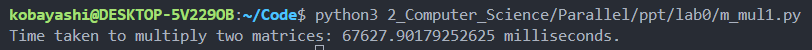
\includegraphics[width=0.8\textwidth]{figures/m_mul1.png}
    \caption{Python实现}
\end{figure}

    \item C/C++实现
\begin{lstlisting}[language=C]
void matrix_multiply(const vector<vector<double>>& A, const vector<vector<double>>& B, vector<vector<double>>& C) {
    int rows_a = A.size();
    int cols_a = A[0].size();
    int rows_b = B.size();
    int cols_b = B[0].size();

    if (cols_a != rows_b) {
        throw invalid_argument("Invalid matrix dimensions");
    }

    C.resize(rows_a, vector<double>(cols_b, 0.0));

    auto start_time = chrono::high_resolution_clock::now();
    for (int i = 0; i < rows_a; ++i) {
        for (int j = 0; j < cols_b; ++j) {
            for (int k = 0; k < cols_a; ++k) {
                C[i][j] += A[i][k] * B[k][j];
            }
        }
    }
    auto end_time = chrono::high_resolution_clock::now();
    auto duration = chrono::duration_cast<chrono::milliseconds>(end_time - start_time);
    cout << "Time taken to multiply two matrices: " << duration.count() << " milliseconds." << endl;
}
\end{lstlisting}
\begin{figure}[H]
    \centering
    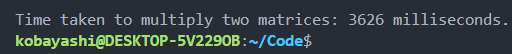
\includegraphics[width=0.8\textwidth]{figures/m_mul2.png}
    \caption{C/C++实现}
\end{figure}

    \item 调整循环顺序
\begin{lstlisting}[language=C]
void matrix_multiply(const vector<vector<double>>& A, const vector<vector<double>>& B, vector<vector<double>>& C) {
    int rows_a = A.size();
    int cols_a = A[0].size();
    int rows_b = B[0].size(); // change B from k*n to n*k
    int cols_b = B.size();

    if (cols_a != rows_b) {
        throw invalid_argument("Invalid matrix dimensions");
    }

    C.resize(rows_a, vector<double>(cols_b, 0.0));

    auto start_time = chrono::high_resolution_clock::now();
    for (int i = 0; i < rows_a; ++i) {
        for (int j = 0; j < cols_b; ++j) {
            for (int k = 0; k < cols_a; ++k) {
                C[i][j] += A[i][k] * B[j][k];
            }
        }
    }
    auto end_time = chrono::high_resolution_clock::now();
    auto duration = chrono::duration_cast<chrono::milliseconds>(end_time - start_time);
    cout << "Time taken to multiply two matrices: " << duration.count() << " milliseconds." << endl;
}
\end{lstlisting}
\begin{figure}[H]
    \centering
    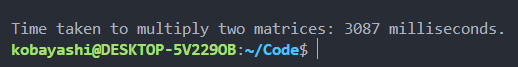
\includegraphics[width=0.8\textwidth]{figures/m_mul3.png}
    \caption{调整循环顺序}
\end{figure}

    \item 编译优化
\begin{figure}[H]
    \centering
    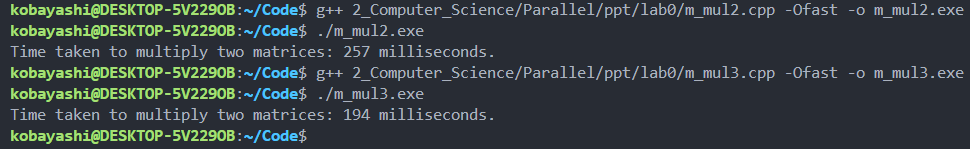
\includegraphics[width=0.8\textwidth]{figures/m_mul4.png}
    \caption{编译优化}
\end{figure}

    \item 循环展开
\begin{figure}[H]
    \centering
    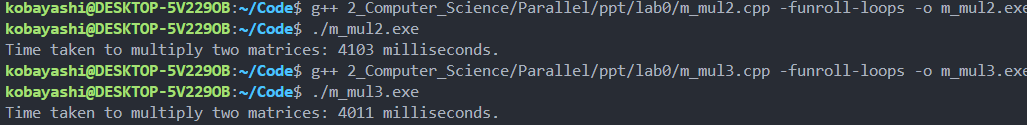
\includegraphics[width=0.8\textwidth]{figures/m_mul5.png}
    \caption{循环展开}
\end{figure}

    \item Intel MKL
\begin{figure}[H]
    \centering
    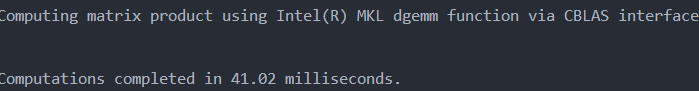
\includegraphics[width=0.8\textwidth]{figures/m_mul6.png}
    \caption{Intel MKL}
\end{figure}

\end{itemize}
\end{document}